\documentclass[
a4paper
]{scrreprt}
\usepackage[ngerman]{babel}
\usepackage[utf8]{inputenc}
\usepackage{textcomp, expdlist, array, colortbl, xcolor}
\usepackage[pdftex]{graphicx}
\usepackage[TS1, T1]{fontenc}
\usepackage{palatino} % Schriftart
\usepackage{parskip} %Erste Zeile eines Paragrafen nicht einrücken

\usepackage{listings}
\usepackage{color}
\usepackage{xcolor}

% Snippets settings
\lstset{language=C++,
	basicstyle=\ttfamily,
	keywordstyle=\color{blue}\ttfamily,
	stringstyle=\color{red}\ttfamily,
	commentstyle=\color{magenta}\ttfamily,
	morecomment=[l][\color{magenta}]{\#}
}


\begin{document}
	\sffamily % Whole document sans-serif
	
	
	% Titelseite
	\begin{titlepage}
		\centering
		
\includegraphics[width=0.8\textwidth]{./images/logo_hska.png}\par\vspace{1cm}
		\vspace{1cm}
		
		{\scshape\Large Systemnahes Programmieren\par}
		\vspace{1.5cm}
		
		{\huge\textbf{Compiler}\par}
		\vspace{2cm}
		
		{\Large\itshape Timo Blust, 48594\par}
		{\Large\itshape Gennadi Eirich, 50629\par}
		{\Large\itshape Tim Essig, 49683\par\par}
		\vspace{2cm}
		
		{\Large\itshape Gruppe 17 (WS 15/16)\par}
		
		\vfill
		
		% Bottom of the page
		{\large \today\par}
	\end{titlepage}
	
	
	% Inhaltsverzeichnis
	\tableofcontents
	
	% Scanner
	\chapter{Scanner}
	\section{Buffer}
	Die Aufgabe der \textit{Buffer}s besteht darin, die Eingabedatei zu puffern.\\
	
	Für die Realisierung der Aufgabe legt der \textit{Buffer} zwei \textbf{char*} an, mir jeweils der Größe von 2048 (\textbf{HSKA\_BUFFER\_SIZE}). 
	Diese werden mit \textbf{posix\_memalign} allokiert und mit \textbf{memset()} auf \textbf{0} gesetzt. Durch das auf \textbf{0} setzen, kann der \textit{Automat} das Ende der Datei erkennen. Folgender code wird für jedes der zwei Buffer (\textbf{\_previousBuffer, \_currentBuffer}) beim instanziieren aufgerufen.
	\begin{lstlisting}
int err = posix_memalign(reinterpret_cast<void**>(buffer), 
HSKA_BUFFER_SIZE, HSKA_BUFFER_SIZE);
memset(*buffer, 0, HSKA_BUFFER_SIZE); // Fill buffer
	\end{lstlisting}
	
	Um das aktuelle Zeichen vom \textit{Buffer} zu bekommen, wird die Methode \textbf{nextChar()} bereitgestellt. Bei jedem Aufruf von \textbf{nextChar()} wird das aktuelle Zeichen aus dem \textit{Buffer} gelesen und einige der folgenden Offsets werden manipuliert.
	\begin{description}
		\item[\_positionOffset] Das absolute Offset des aktuellen Zeichen (wird bei jedem abgefragten Zeichen inkrementiert)
		\item[\_currentColumnNum] Die aktuelle Spalte des Zeichens. Bei einem Zeilenumbruch wird dieses wieder auf \textbf{1} gesetzt.
		\item[\_filePositionOffset] Offset der Datei. Beim einlesen eines neuen Teils der Datei wird dieser um die Größe des eingelesenen buffers erhöht. 
	\end{description}
	
	Ist \textbf{\_positionOffset} gleich \textbf{\_filePositionOffset}, so ist das Ende des aktuellen \textit{Buffer}s erreicht und es muss ein neues Teil der Eingabedatei mit der Länge \textbf{HSKA\_BUFFER\_SIZE} eingelesen werden.
	\begin{lstlisting}
ssize_t size = read(_fileHandle, _currentBuffer, 
			HSKA_BUFFER_SIZE);
	\end{lstlisting}
	
	\begin{center}
		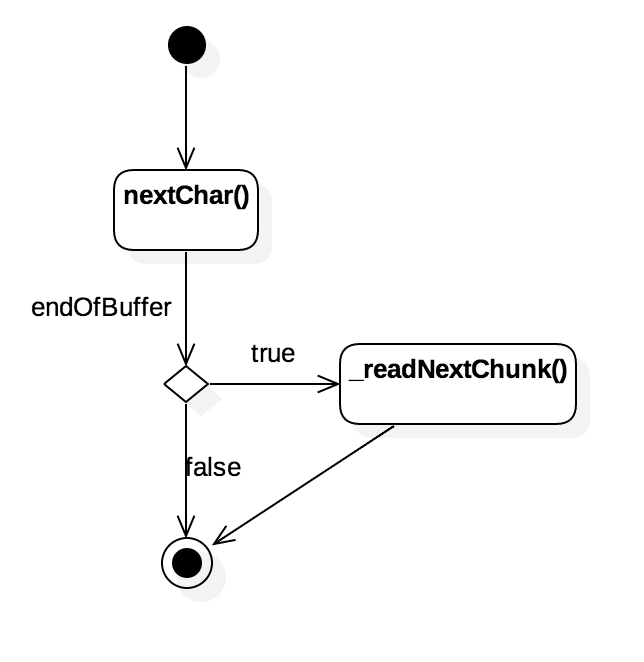
\includegraphics[width=0.5\textwidth]{./images/buffer_activity.png}
	\end{center}
	
	Um die Lexeme und Zahlen bestimmen zu können wird ein kompletter \textit{String} benötigt. Dafür stellt der \textit{Buffer} die Methode \textbf{subString()} bereit. Dieser werden Länge und Offset des geforderten \textit{String}s übergeben.
	Ist der geforderte \textit{String} länger als der Offset (relative Position des letzten Zeichen) des \textbf{\_currentBuffer}, so wird auch aus dem \textbf{\_previousBuffer} gelesen.
	
	
	\section{Symboltabelle}
	Die Aufgabe der Symboltabelle ist es, die gefundenen \emph{Identifier} zu verwalten. In ihr werden die gefundenen \emph{Identifier} in einer HashMap abgelegt und lassen sich schnell wieder finden. Dies ist entscheidend für die Performance des Compilers. \\
	Die Architektur der Symboltabelle ist im folgenden Diagramm dargestellt.
	
	\begin{center}
		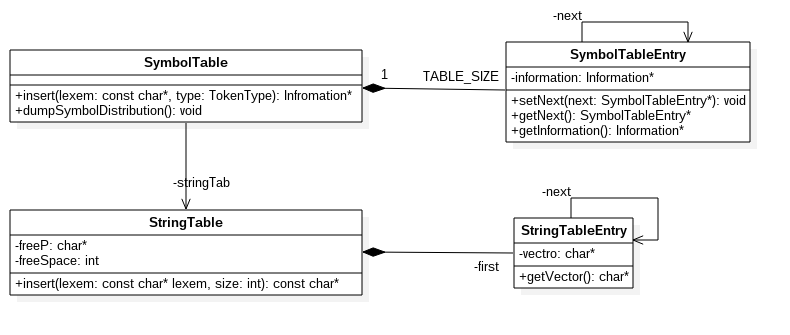
\includegraphics[width=0.8\textwidth]{./images/symtable_class.png}
	\end{center}
	
	Die Hauptkomponente ist die Klasse SymbolTable, diese bietet eine Funktion \emph{Information* insert(const char* lexem, TokenType type)}. Diese Funktion wird vom Scanner jedes mal aufgerufen, wenn er einen neuen \emph{Identifier} findet. Die SymbolTable erzeugt aus dem übergebenen \emph{lexem} den dazu gehörigen Hash und schaut in der Hash-Tabelle nach, ob bereits ein oder mehrere Einträge existieren. Ist dies der Fall, muss kein neuer Eintrag(SymbolTableEntry) angelegt werden und es wird der Zeiger auf das entsprechende \emph{Information}-Objekt zurück gegeben.\\
	
	Wird in der Hash-Tabelle jedoch kein passender Eintrag gefunden, so wird zunächst das Lexem in der StringTable gespeichert(diese erweitert ihren genutzten Speicherplatz bei Bedarf selbst). Für das nun in der StringTable verwaltete Lexem wird nun ein \emph{Information}-Objekt erzeugt, welchem ebenfalls der angegeben TokenType übergeben wird. Es ist damit für den Scanner irrelevant, ob der \emph{Identifier}, welchen er in der SymbolTabelle ablegen möchte, zum ersten oder zum wiederholten mal gefunden wurde.\\
	Der vom Scanner daraufhin erzeugte Token, enthält nun einen Zeiger auf das \emph{Information}-Objekt.
	
	\begin{center}
		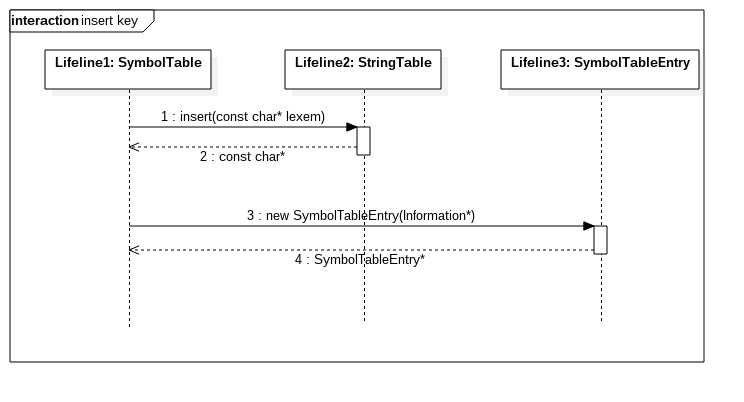
\includegraphics[width=0.8\textwidth]{./images/symtable_seq.png}
	\end{center}    
	
	\subsection*{Verteilung der HashKeys}
	Das Ziel einer guten HashFunktion ist es, dass die HashKeys möglichst gleichmäßig verteilt werden, um die Anzahl der Kollisionen und damit die Anzahl der nötigen genauen String-Vergleiche möglichst gering zu halten.\\
	
	Allerdings darf die Berechnung HashKeys wiederum nicht zu aufwendig sein, da eine Langsame HashFunktion ebenfalls einen negativen Einfluss auf die Performance hätte.\\
	Die HashKeys werden in der SymbolTabelle wie folgt berechnet:\\
	\pagebreak
	\begin{lstlisting}
unsigned int SymbolTable::hash(char const* lexem)
{
 unsigned int h = 0;
	
 while( *lexem != 0)
 {
  h = 31*h + *lexem;
  lexem++;
 }
	
 return h % TABLE_SIZE;
}
	\end{lstlisting}
	
	
	Das unten stehende Diagramm zeigt die Verteilung der Einträge pro HashKey bei einem sehr großen Dokument(ca. 20.000 \emph{Identifier}). 
	\begin{center}
		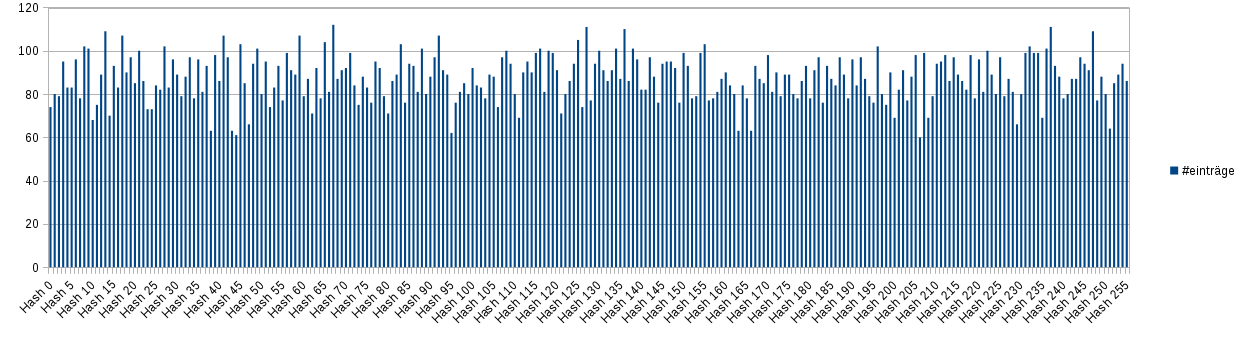
\includegraphics[width=\textwidth]{./charts/hashtable_distribution.png}
	\end{center}
	Es ist gut zu erkennen, dass die Anzahl der Einträge pro HashKey(die HashTable hat eine Größe von 256 Keys) relativ gleichmäßig verteilt sind.\\
	Damit scheint die HashFunktion unseren Anforderungen zu genügen, nicht zu teuer zu sein und trotzdem möglichst gleich verteilte Werte zu liefern.
	
	    \section{Automat}
	Die Aufgabe des Automaten ist es, anhand der Eingabe (in diesem Fall des Quellcodes) gültige und ungültige Tokens zu erkennen.
	
	\subsection{TokenScanner}
	Zu jedem Token gehört ein Automat, welcher nur für die Erkennung dieses spezifischen Tokens sorgt. Zur Verwaltung der Automaten wurde eine darüber liegende Ebene geschaffen, welche durch den \textbf{TokenScanner} abgebildet wird.
	\begin{center}
		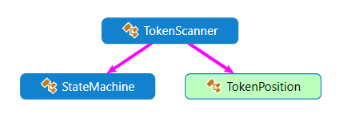
\includegraphics{./images/tokenscanner_dependency.png}		
	\end{center}
	\begin{center}		
		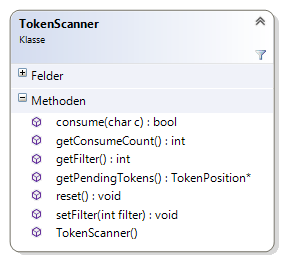
\includegraphics{./images/tokenscanner_cd.png}
	\end{center}
	Ein Aufruf von \textit{consume(char c)} leitet das Zeichen \textit{c} an alle Automaten weiter. Anschließend wird geprüft, ob ein Automat das Zeichen akzeptiert. Hat kein Automat das Zeichen akzeptiert, wird ein \textit{ERROR} Token erstellt. Wurde das Zeichen jedoch akzeptiert, wird geprüft, ob sich ein Automat in einem finalen Zustand befindet. Dies würde bedeuten, dass ein neues Token gefunden wurde. Alle gefundenen Tokens werden in einer doppelt verlinkten Liste gespeichert. Als Listenelement dient hier die Klasse \textbf{TokenPosition}.	Hier werden Tokentyp, die Größe des Tokens (Anzahl der Zeichen), die absolute Position (seit beginn der Eingabe), sowie die relative Position zur aktuellen Eingabe gespeichert.
	
	Mithilfe der Funktionen \textit{TokenPosition::getNext()} und \textit{TokenPosition::getPrevious()} lassen sich das nächste, bzw. das vorherige Element ermitteln. Gibt eine der beiden Funktionen einen \textbf{nullptr} zurück, wurde das Ende, bzw. der Anfang der Liste erreicht.
	\begin{center}		
		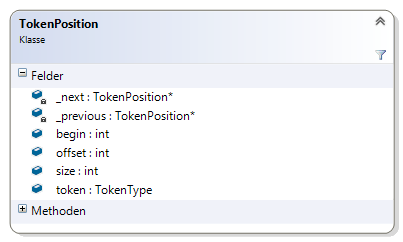
\includegraphics{./images/tokenposition_cd.png}
	\end{center}
	Durch einen Aufruf der Methode \textit{TokenScanner::getPendingTokens()} erhält man sämtliche Tokens, die seit dem letzten Aufruf von \textit{TokenScanner::getPendingTokens()} gefunden wurden.
	
	\subsection{StateMachine}
	Die Klasse \textbf{StateMachine} bildet den eigentlichen Automaten ab. Das folgende Abhängigkeitsdiagramm zeigt den groben Aufbau der \textbf{StateMachine}. Die Zustände des Automaten werden von 0 bis n durchnummeriert, wodurch keine beschreibende Klasse nötig ist.
	\begin{center}		
		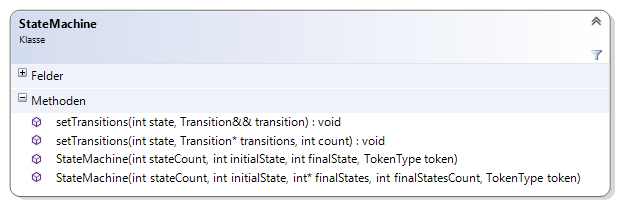
\includegraphics[width=\linewidth]{./images/statemachine_cd.png}
	\end{center}
	Der Konstruktor der \textbf{StateMachine} benötigt die Anzahl der Zustände, den Index des Startzustands, eine Auflistung der Endzustände und den \textbf{TokenType}, welcher dem Automat zugeordnet werden soll.
	
	Der Automat kann eine beliebige Anzahl an Transitionen aufnehmen.  
	\begin{center}		
		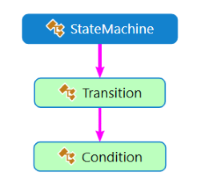
\includegraphics{./images/statemachine_dependency.png}
	\end{center}
	Die Klasse \textbf{Transition} beschreibt eine Transition. In ihr wird der Zielzustand und die Transitionsbedingung abgelegt. Eine Transitionsbedingung wird durch die abstrakte Klasse \textbf{Condition} dargestellt. Diese stellt die Methode \textit{accepts(char input)} bereit, welche \textit{true} zurück gibt, wenn \textit{input} die Bedingung erfüllt.
	\begin{center}		
		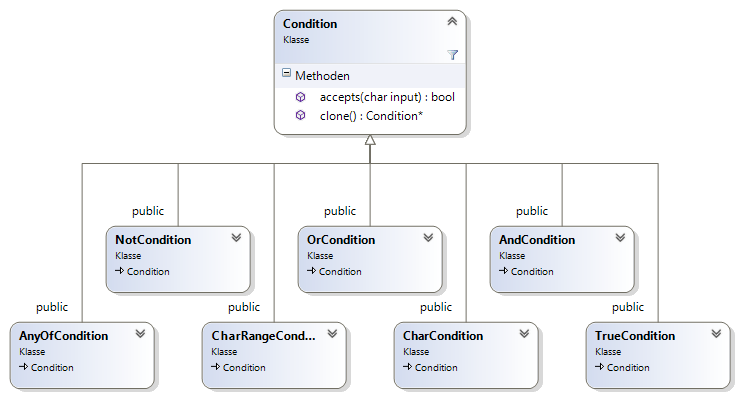
\includegraphics[width=\linewidth]{./images/condition_cd.png}
	\end{center}
	Die drei Ableitungen \textbf{NotCondition}, \textbf{OrCondition} und \textbf{AndCondition} implementieren die Negation und die logischen Operatoren Oder und Und. Sollen z.B. nur alphanumerische Zeichen akzeptiert werden, kann die Bedingung wie folgt implementiert werden:	 
	\begin{lstlisting}
auto alphanumerical = new OrCondition(
	new CharRangeCondition('0', '9'),
	new CharRangeCondition('a', 'z'), 
	new CharRangeCondition('A', 'Z'));
	\end{lstlisting}
	Da viele Tokens aus nur einem Zeichen bestehen, benötigen die zugehörigen Automaten auch nur zwei Zuständen und eine Transition. Um die Initialisierung eines solchen Automaten zu erleichtern, steht die Methode \textit{StateMachine::createAtomic(Token::TokenType token, Condition* condition)} zur Verfügung. Der folgende Codeausschnitt aus der Datei '\textit{state-machine/TokenScanner.cpp}' zeigt die Initialisierung der Automaten für die größer, kleiner und gleich Token:
	\begin{lstlisting}
_sms[8] = StateMachine::createAtomic(
	Token::GREATER, new CharCondition('>'));
_sms[9] = StateMachine::createAtomic(
	Token::LESS, new CharCondition('<'));
_sms[10] = StateMachine::createAtomic(
	Token::EQUAL, new CharCondition('='));
	\end{lstlisting}
	
	
	
	\section{Scanner}
	Die Aufgabe des \textit{Scanner}s ist dem Aufrufer das nächste \textit{Token} der Eingabedatei zu übergeben und dieses unter Umständen in die \textit{Symboltabelle} einzutragen.\\
	
	Beim Aufruf von \textbf{nextToken()} hold der \textit{Scanner} das nächste Zeichen vom \textit{Buffer} und übergibt es dem Automaten. Wird dabei ein \textit{Token} erkannt, so gibt die Methode des \textit{Automaten} \textbf{true} zurück.
	
	Wird ein \textbf{IDENTIFIER} erkannt so wieder dessen \textit{String} bestimmt und dieser wird in die \textit{Symboltabelle} eingetragen. Diese, vom Aufruf zurückgegebene \textit{Information}, wird dem \textit{Token} angehängt.
	
	Im Falle eines \textbf{INTEGER} wird ebenso dessen \textit{String} bestimmt und der Wert der Zahl mit \textbf{strtol} bestimmt. Dabei wird überprüft ob die Zahl im Zahlenbereich liegt. Falls nicht, wird ein Fehler auf \textbf{stderr} ausgegeben.
	
	Bei einem gefunden \textbf{ERROR} wird dieses auf \textbf{stderr} ausgegeben mit Zeile, Spalte und dem Symbol.
	
	Alle anderen \textit{Token} werden direkt dem Aufrufer zurückgegeben. 
	
	Des weiteren enthält jedes \textit{Token} die Informationen Typ, Zeile und Spalte.
	
	\begin{center}
		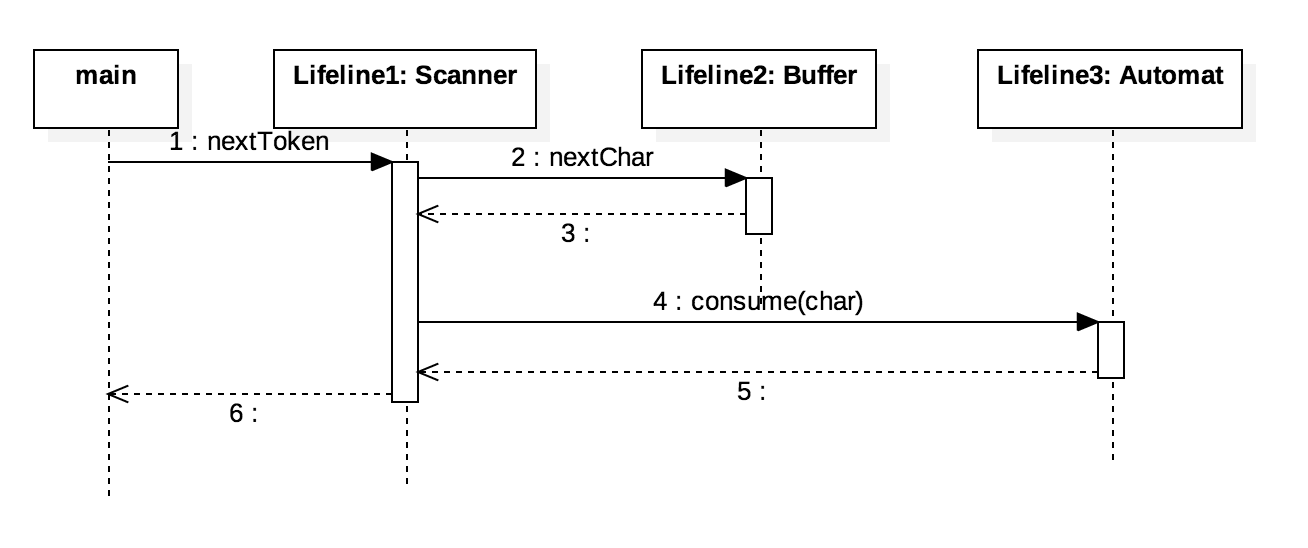
\includegraphics[width=0.8\textwidth]{./images/scanner_sequence.png}
	\end{center}
	
	Unter gewissen Umständen kann es auch passieren, dass der \textit{Automat} mehrere \textit{Token}s zurückgibt. Dabei wird überprüft ob weitere \textit{Token} an diesem anhängen. Falls dem so ist werden diese lokal abgelegt und beim nächsten Aufruf von \textbf{nextToken()} priorisiert abgearbeitet.
	
	Folgend der Code für das Überprüfen, ob weitere \textit{Token} dem aktuellen anhängen. Da das \textbf{NEW\_LINE}-Token ignoriert wird, wird dieses gelöscht und es wird weiter geprüft. Sollte das nächste ein \textbf{nullptr} sein, so ist das Ende der Liste erreicht und es gibt keine weiteren \textit{Token} mehr. Ab jetzt kann wieder ein Zeichen aus dem \textit{Buffer} eingelesen werden.
	
	\begin{lstlisting}
void Scanner::_checkForPendingToken(TokenPosition* tokens)
{
 auto next = tokens->getNext();
 if (next == nullptr)
 {
  _pendingTokens = nullptr;
  return;
 }
	
// Ignore the NEW_LINE token
if (next->token == Token::TokenType::NEW_LINE)
{
 _checkForPendingToken(next); // Check next one for pending token
 delete next; // delete it because its never used/ignored
}
else
 _pendingTokens = next;
}
	\end{lstlisting}
	
	
	\section{Ausführung}
	Für die Ausführung müssen dem Programm zwei Parameter übergeben werden.
	
	\begin{enumerate}
		\item Eingabedatei (Sourcecode)
		\item Ausgabedatei (Aufistung aller gefundenen \textit{Token}s)
	\end{enumerate}
	
	Gebaut wird das Programm mit \textbf{Makefile}.
	
	Folgend die Kommandos für den Bau und die Ausführung des Scanners.
	
	\begin{lstlisting}
$ make 			// im root Ordner
$ cd bin/		// Ordner in dem das target liegt
$ ./HsKA-Scanner eingabedatei.txt ausgabedatei.txt
	\end{lstlisting}
	
	% Parser
	%	\chapter{Parser}
	
\end{document}